\documentclass[a4paper]{article}
\usepackage[utf8]{inputenc}
\usepackage{textcomp}
\usepackage{geometry}
\geometry{ left=2cm, right=2cm, top=2cm, bottom=2cm, bindingoffset=5mm}
\usepackage{graphicx}
\usepackage{xcolor}
\usepackage{hyperref}
\date{}
\author{}
\usepackage{fancyhdr}
\pagestyle{fancy}
\fancyhf{}
\fancyhead[R]{2973140 - Felix Bühler \\ 2892258 - Gerhard Breul \\  3141241 - Jamie Ullerich}
\fancyhead[L]{Information Visualisation and Visual Analytics \\ WS 2019/20 }
\renewcommand{\headrulewidth}{0.5pt}
\usepackage{tikz}
\usetikzlibrary{calc}
\usepackage{amsmath}
\usepackage{cleveref}
\usepackage{subcaption}

\usepackage{changepage,titlesec}
\titleformat{\section}[block]{\bfseries}{\thesection.}{1em}{}
\titleformat{\subsection}[block]{}{\thesubsection}{1em}{}
\titleformat{\subsubsection}[block]{}{\thesubsubsection}{1em}{}
\titlespacing*{\subsection} {2em}{3.25ex plus 1ex minus .2ex}{1.5ex plus .2ex}
\titlespacing*{\subsubsection} {3em}{3.25ex plus 1ex minus .2ex}{1.5ex plus .2ex}
\setcounter{MaxMatrixCols}{20}

\title{\textbf{Assignment 11}}

\begin{document}
\maketitle 
\thispagestyle{fancy}

\section*{Task 1 - Geographical Visualization}
\subsection*{a)} The main challenge with map projection is having to map a three-dimensional space (in this case, the surface of a sphere) onto a two-dimensional one without distorting crucial information. Map projections can be categorized according to which property of the sphere they represent is preserved, such as preservation of certain distances (equidistant), angles (conformal), and areas (equal-area).
\subsection*{b)} Tissot’s indicatrix is used to visualize distortions of map projections. Each area represents a circle of fixed size on the globe. 
For the Mercator projection, these areas will maintain their original round form  but become bigger towards the poles, demonstrating a preservation of angles and a distortion of area.
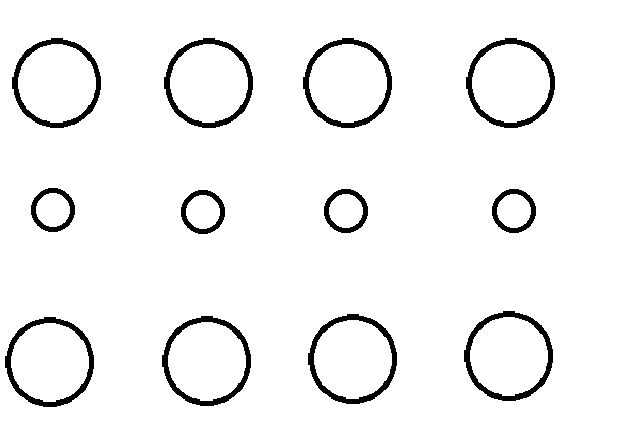
\includegraphics[width=0.7\linewidth]{Mercator} \\
Tissot’s indicatrix of the Cassini projection shows that there is no distortion for points along the central axis, however, the further a point is away from the poles, the stronger the distortion becomes, in terms of size as well as angle.
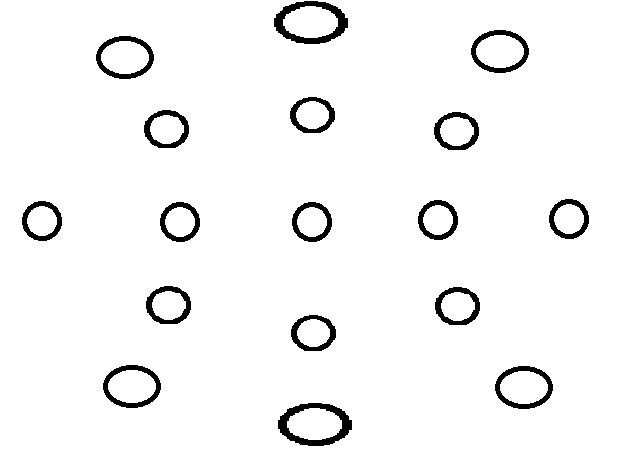
\includegraphics[width=0.7\linewidth]{Cassini}\\
\subsection*{c)}
\subsection*{d)}
\subsection*{e)}

\section*{Task 2 - Kernel Density Estimation}
\begin{figure}[th!]
	\centering
	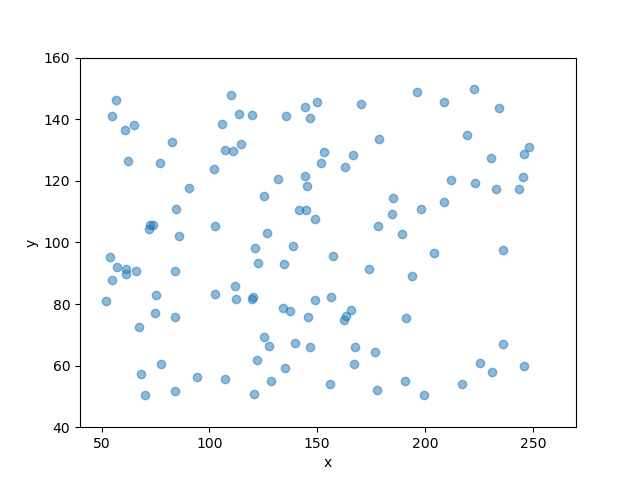
\includegraphics[width=0.7\linewidth]{scatter}
	\caption{scatter-plot}
	\label{fig:scatter}
\end{figure}

\begin{figure}[th!]
	\centering
	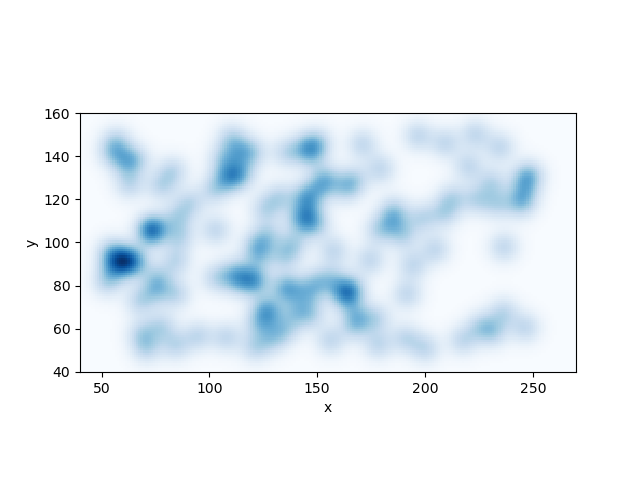
\includegraphics[width=0.7\linewidth]{density}
	\caption{kernel density estimation}
	\label{fig:density}
\end{figure}


\end{document}
